	\begin{Huge}
			Informatik
		\end{Huge}
		\begin{exampleblock}{\textcolor{white}{Was ist der Studiengang?}}
			Der grundständigste *-Informatik-Studiengang. Beinhaltet im Gegensatz zu anderen Studiengängen den meisten Umfang an technischer und theoretischer Informatik. Eine gute Portion Mathe ist außerdem dabei. Außerdem beinhaltet die Informatik ein beliebig wählbares Schwerpunktfach (das nicht Sport sein darf). Danach kann das Studium mit einem Master \\ (4 Semester Regelstudienzeit) weitergeführt werden.
		\end{exampleblock}
	\begin{block}{Welcher Teil macht wie viel im Studium aus?}
		\begin{figure}[h!]
			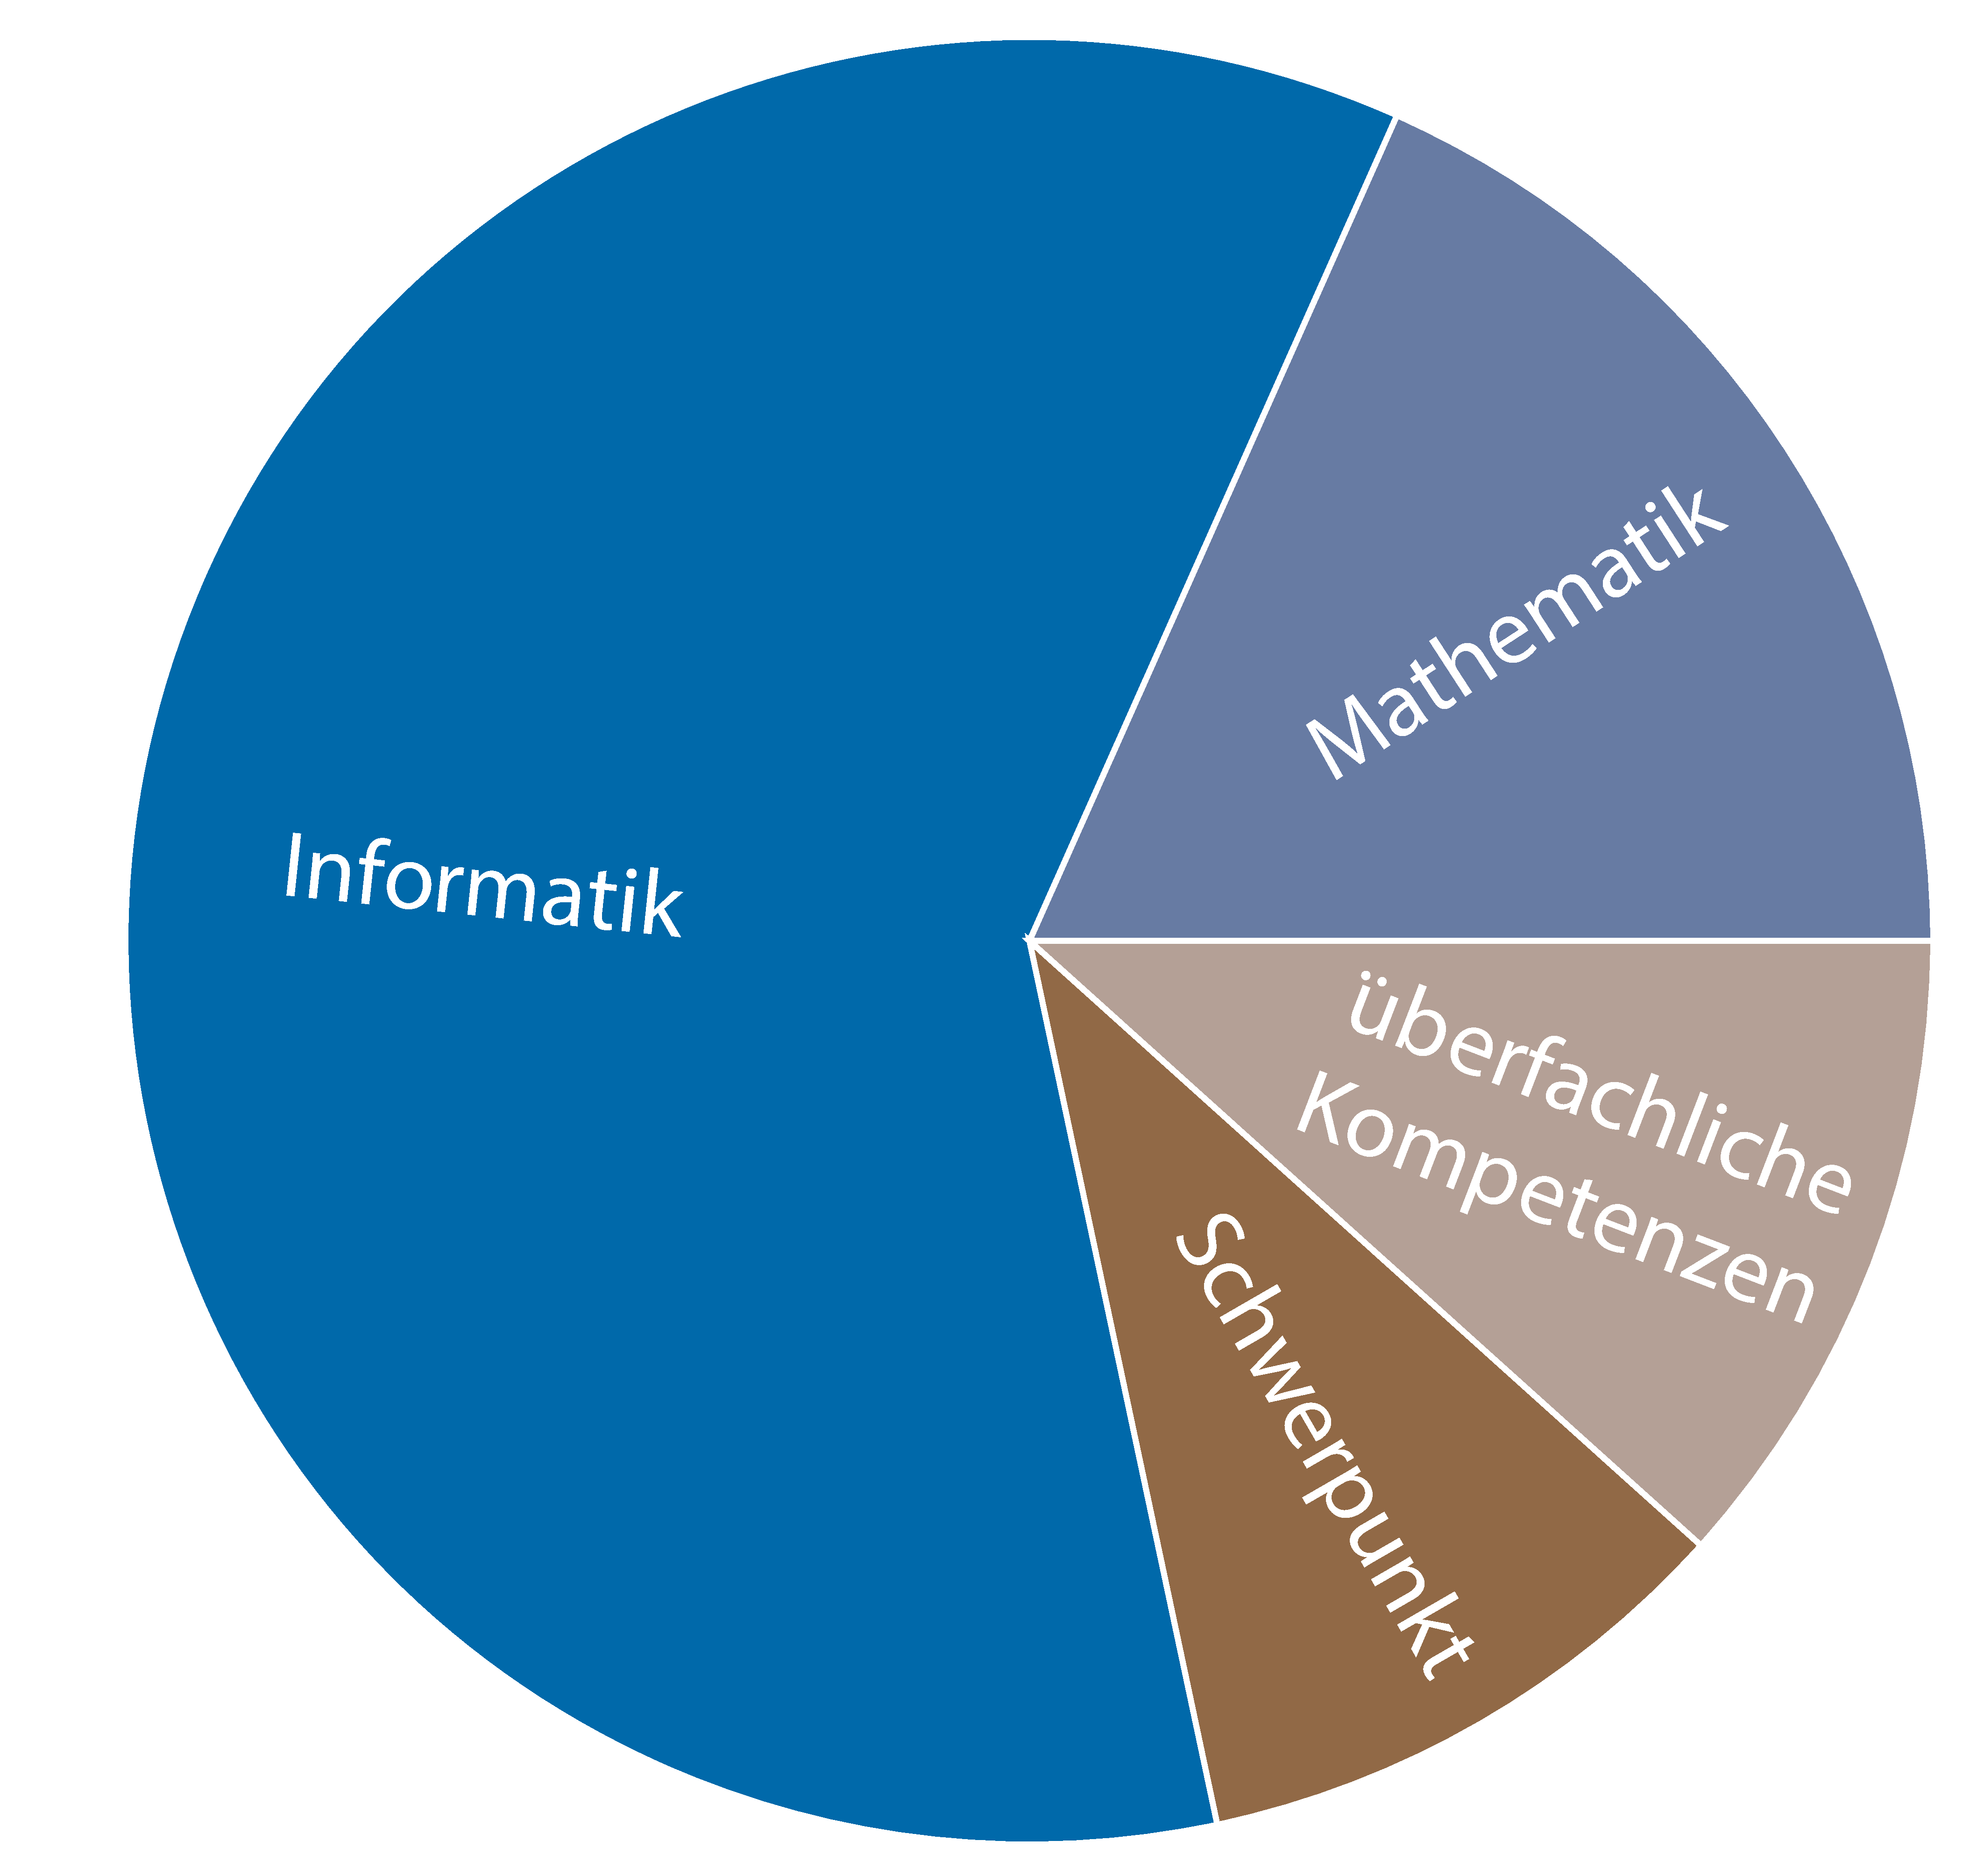
\includegraphics[width=0.4\textwidth]{charts/informatik-Piechart.pdf}
			\caption{Verteilung der Themenbereiche über das komplette Studium}
		\end{figure}
	\end{block}
	\begin{block}{Was macht man in welchem Semester?}
		\begin{figure}[h!]
			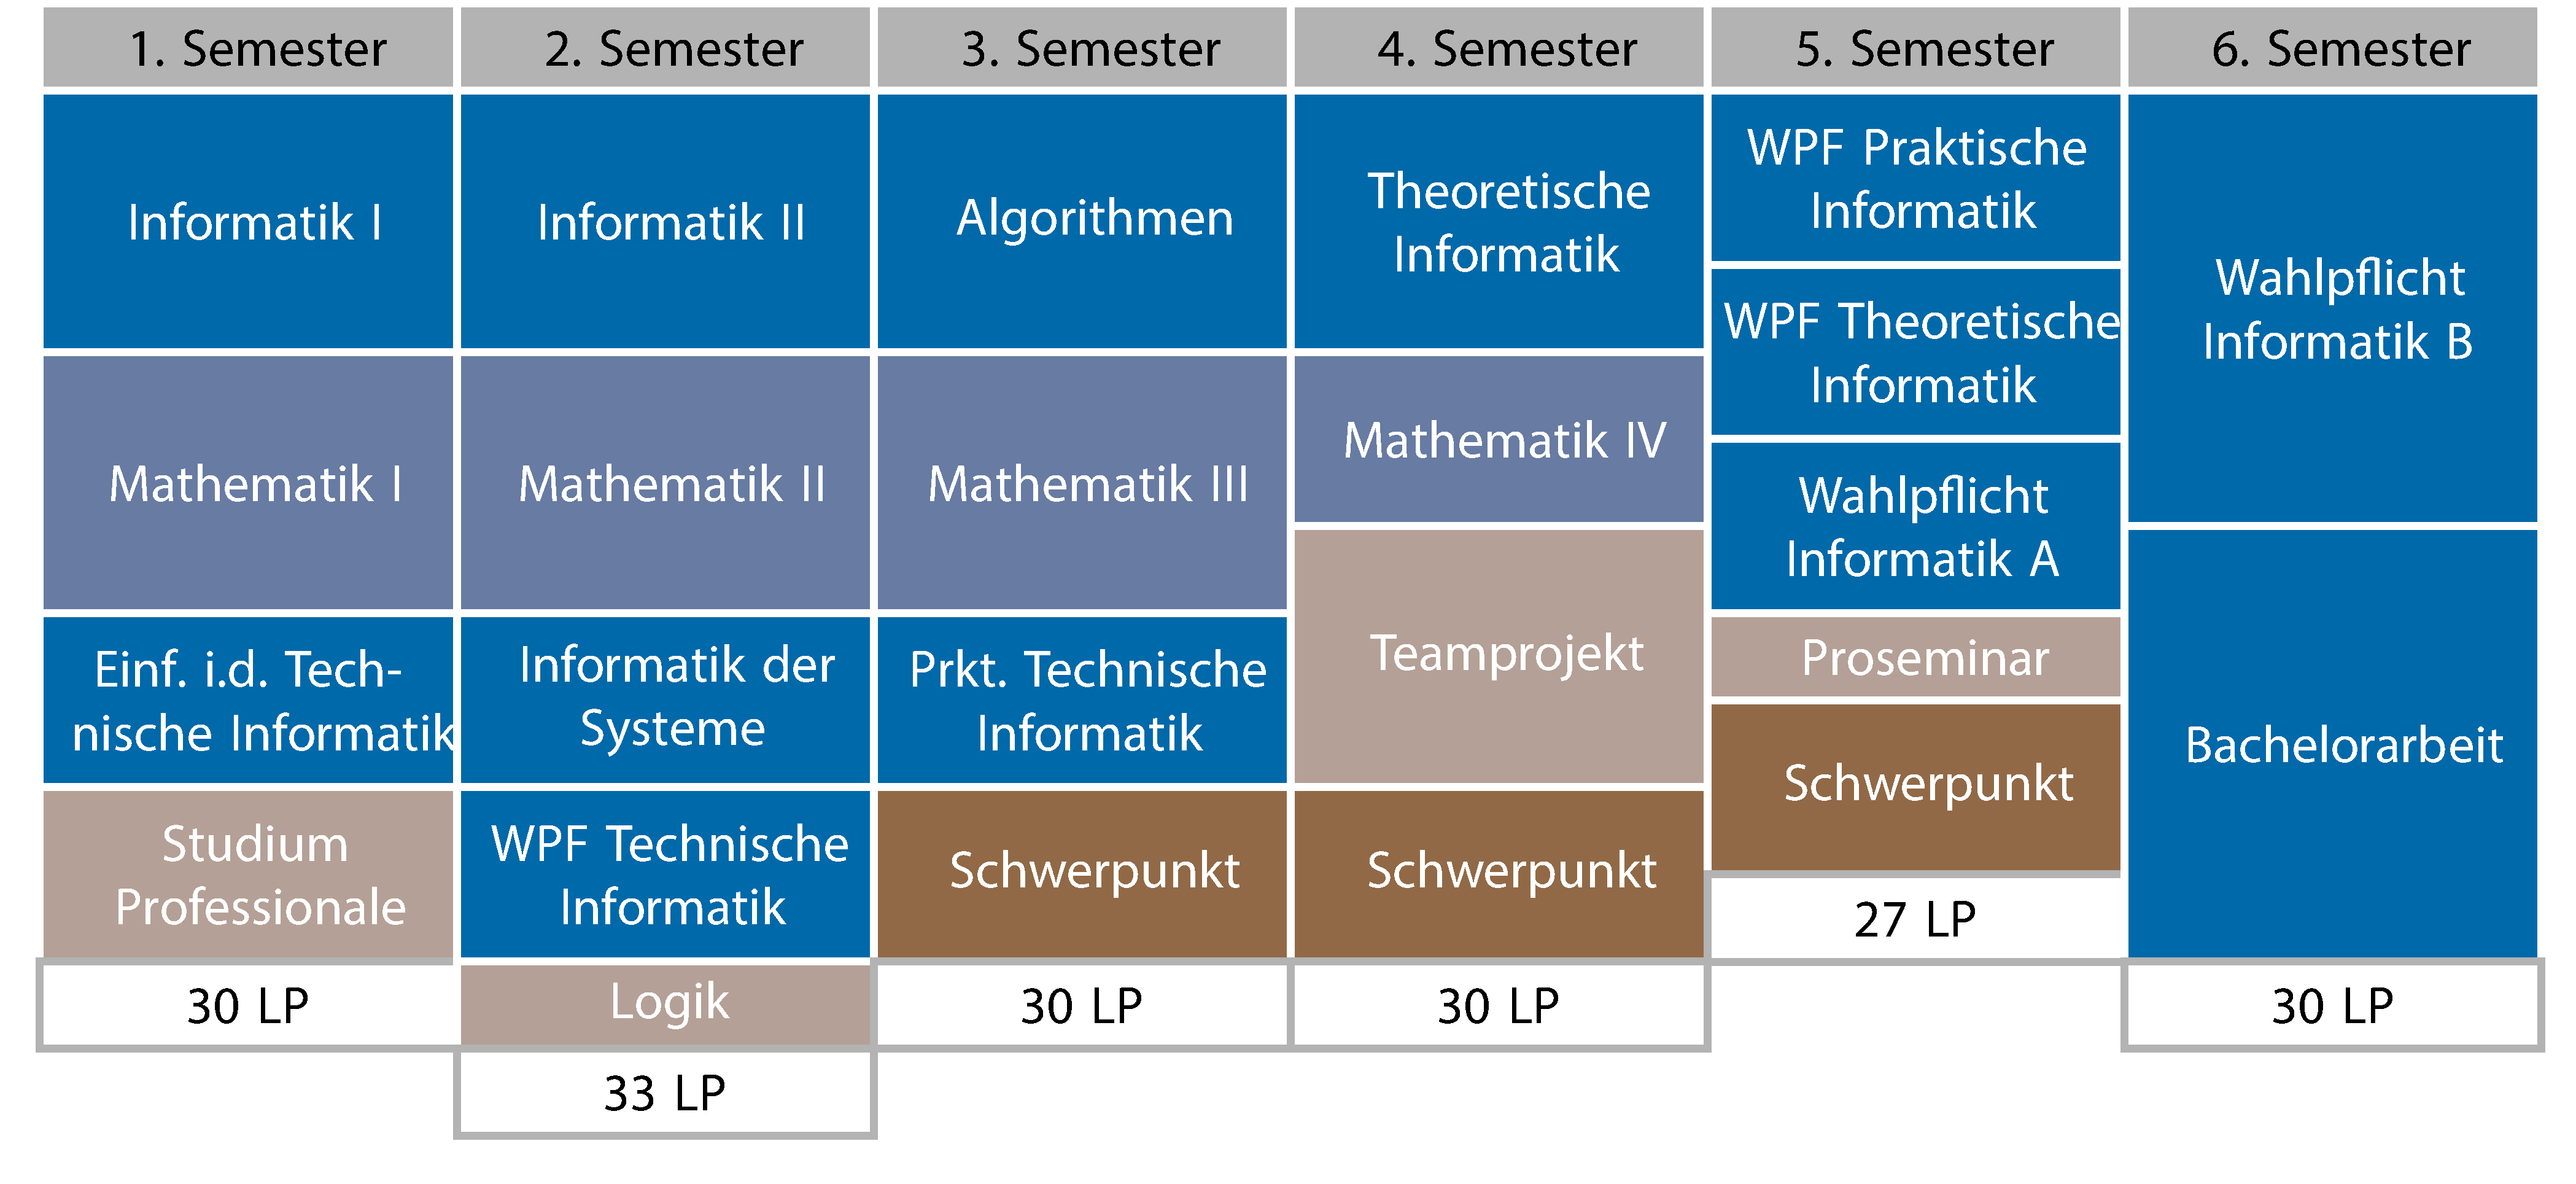
\includegraphics[width=\textwidth]{charts/informatik-Studienplan_abWS18.pdf}
		\end{figure}
		Das 1. Semester ist nach Plan ein Wintersemester. Wenn du dein Studium zum Sommersemester beginnen möchtest, beginnst du im Plan bei Semester 2 und machst dann Semester 1. 
		Dieser Verlauf ist unabhängig vom Studienbeginn nur ein Vorschlag und kein bindender Studienplan. Es empfiehlt sich jedoch, den Plan einzuhalten, wenn man in Regelstudienzeit studieren möchte.
	\end{block}
\vfill
\begin{flushright}
	
\includegraphics[width=0.4\textwidth]{fsilogo.pdf}
\end{flushright}
